\documentclass{beamer}
\usetheme{Oxygen}
\usepackage{verbatim}
\usepackage{minted}

\title{Automated Code Transformation for Distributed Training of TensorFlow ML Models}
\author{Yusung Sim\inst{1}, Wonho Shin\inst{1}, Sungho Lee\inst{2}}
\institute{
  \inst{1}%
  School of Computing, KAIST
  \and
  \inst{2}%
  Department of Computer Science and Engineering,\\ 
  Chungnam National University
}
\date{2022}

\begin{document}
% 0. Title
\frame{\titlepage}


% 1. Introduction
\begin{frame}{Reducing ML Training Time}
  Reducing the \textbf{training time} is an 
  important factor in ML development.\\
  
  Takes longer time than traditional development.

  \begin{itemize}
    \item Simple CNN-based classifier for MNIST trains in \textbf{2-3 hours}
    \item AlphaGo trained for \textbf{3 weeks} (even with 50 GPUs)
    \item Training BERT model in single TPU takes over \textbf{1.5 month}
  \end{itemize}

  Training time is bottleneck in the deployment loop.

  \begin{itemize}
    \item Evaluation is done after the tranining is complete
    \item Development speed cannot catch up increasing size of dataset 
  \end{itemize}
\end{frame}


\begin{frame}{Distributed ML Training}
  \textbf{Distributed Training} technique can reduce the training time

  \begin{definition}
    \textit{Distributed training} is a ML training technique
    that\\distributes the training workload over multiple hardware devices
    (GPUs, TPUs, etc). 
  \end{definition}
  \begin{figure}
    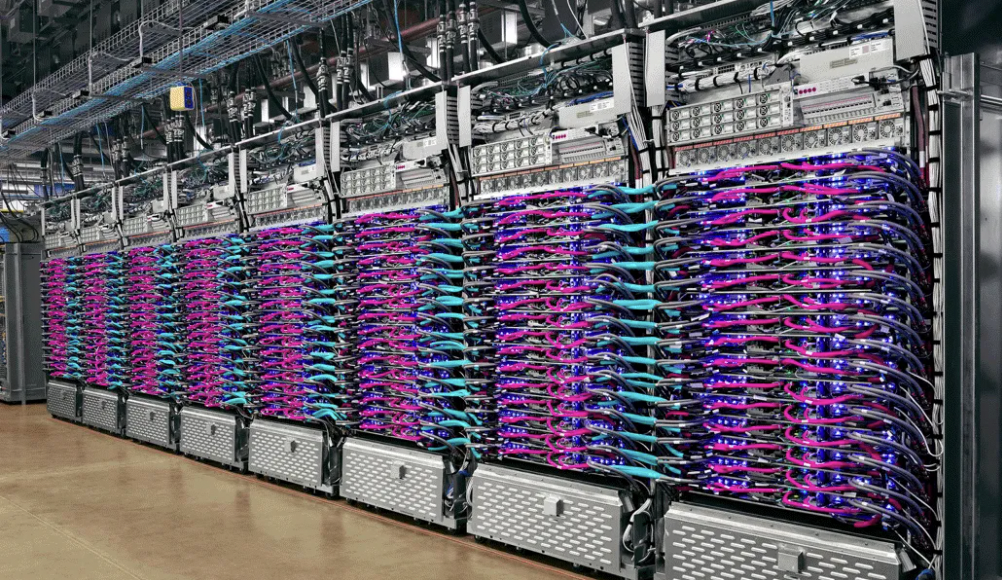
\includegraphics[height=35mm]{TPU}
    \\ {\tiny TPUs - Google Cloud}
  \end{figure}
\end{frame}

\begin{frame}{Distributed ML Training: Data-parallel Approach}
  \begin{figure}
    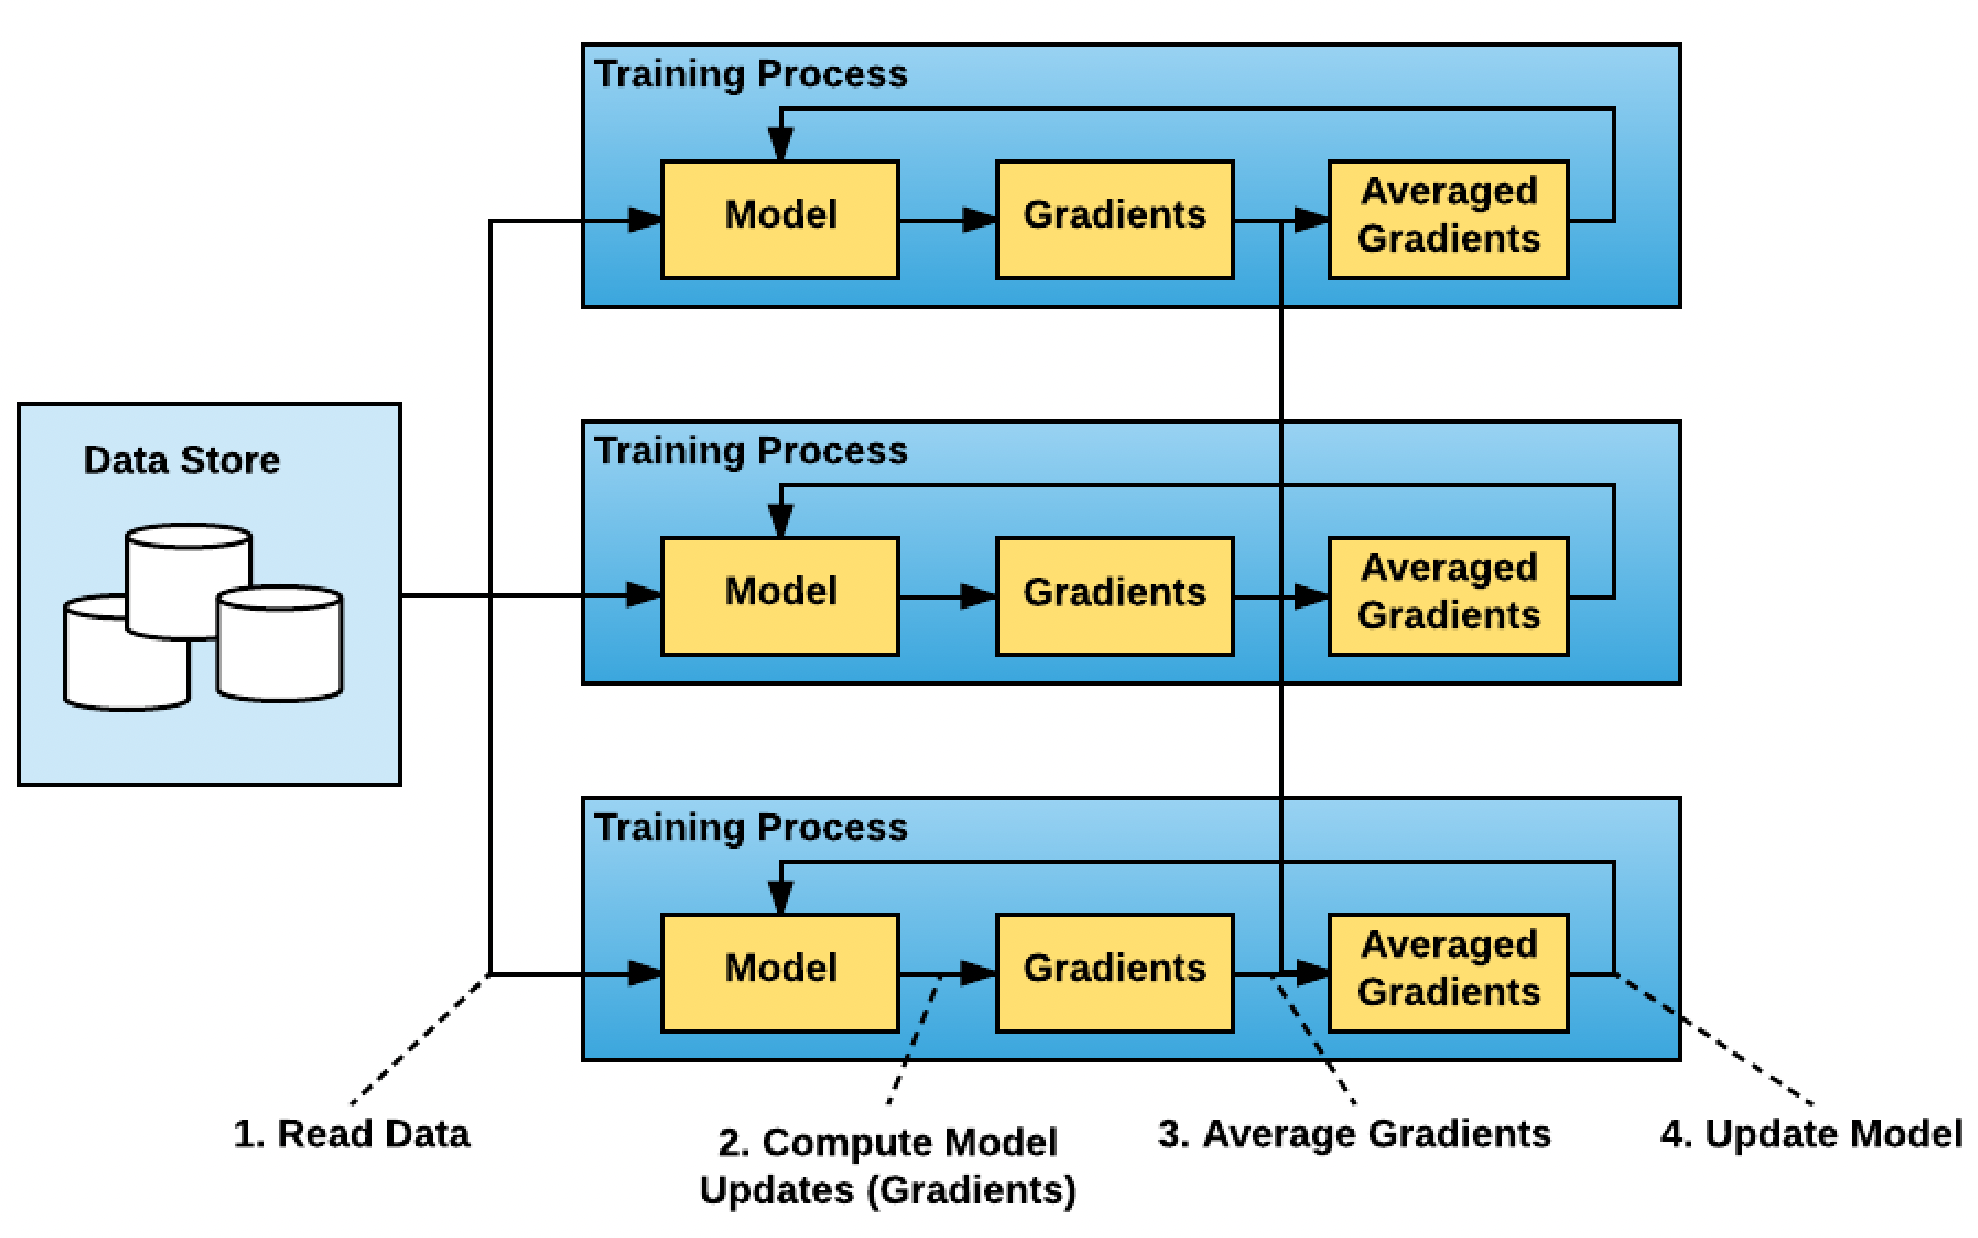
\includegraphics[height=50mm]{data-parallel}
  \end{figure}
  {\footnotesize
  \begin{itemize}
    \item Multiple instances of the model assigned to each device.
    \item Train dataset is divided by the number of devices, assigned to each.
    \item Gradients are averaged before applied to the model.
  \end{itemize} 
  }
\end{frame}

\begin{frame}[fragile]{Horvod: Distributed Training Framework}
  Distributed training code is often written in \textbf{Horovod},\\
  a data-parallel distributed training framework for Python. 
  \begin{figure}[!h]
    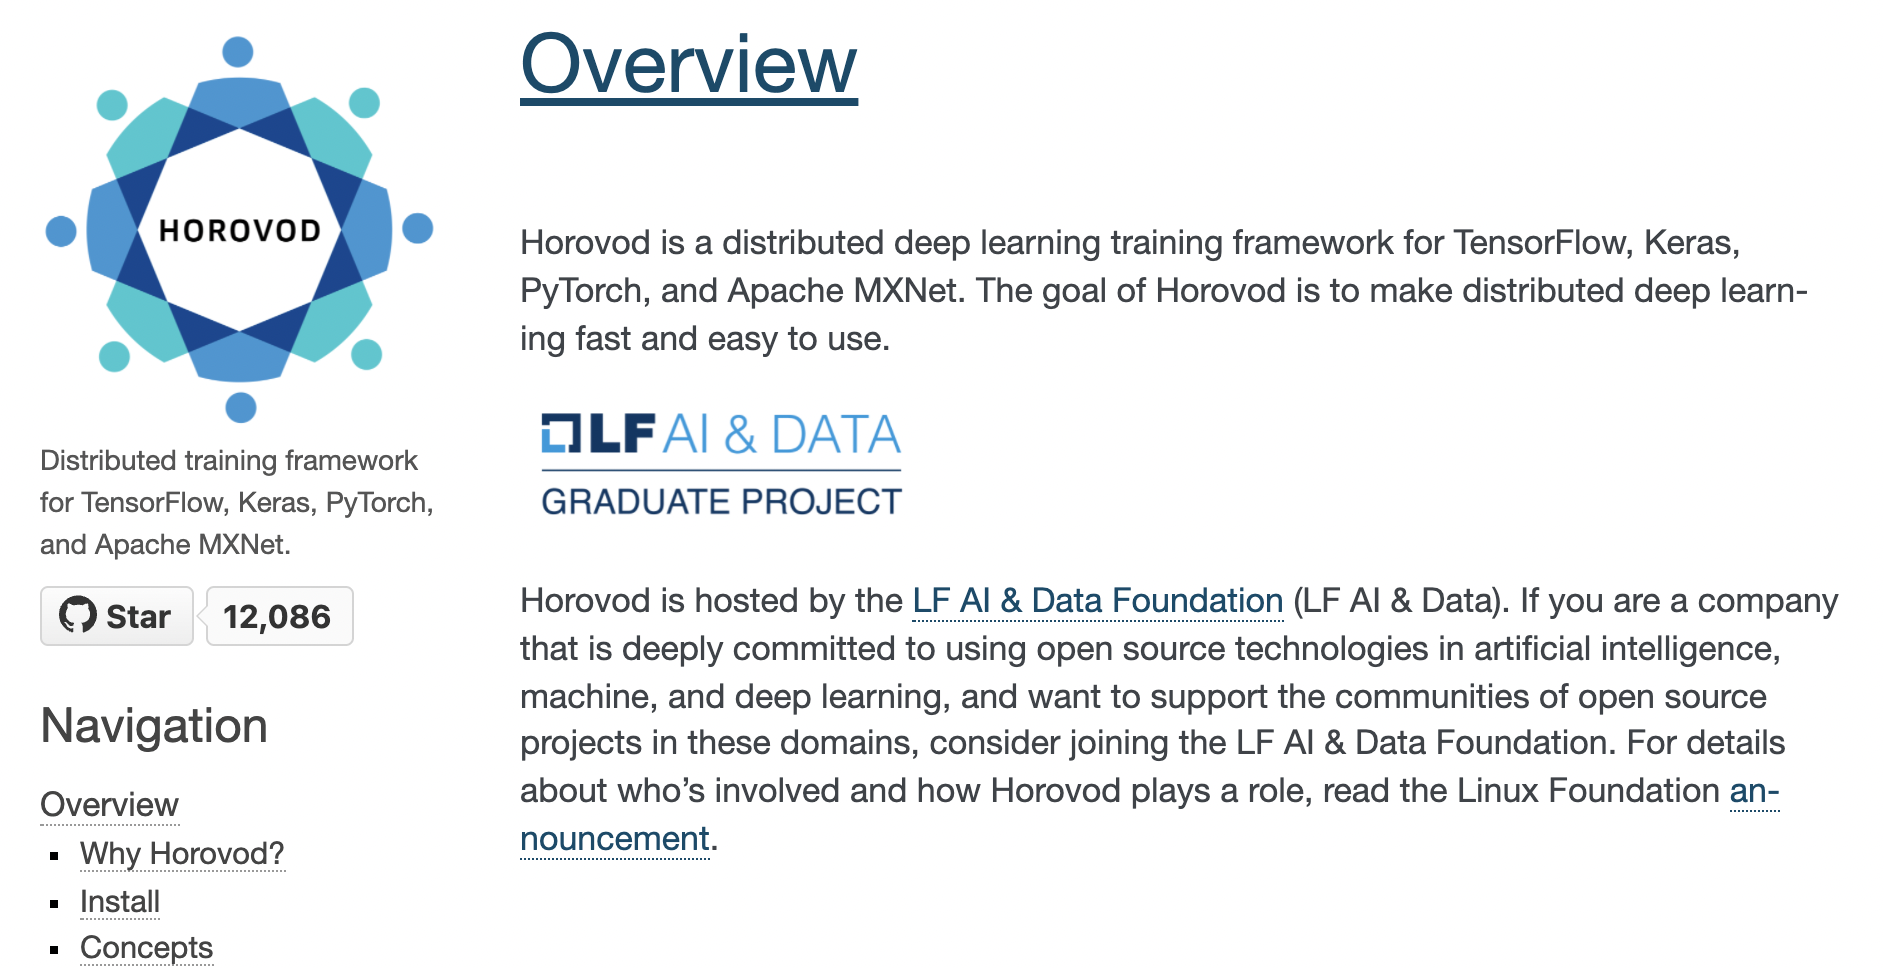
\includegraphics[height=55mm]{horovod_logo}
  \end{figure}
\end{frame}


\begin{frame}{Single GPU Training Code to Distributed Training Code}
  \begin{columns}[t]
    \begin{column}{.5\textwidth}
      {\tiny
        \inputminted{Python}{tensorflow_ex.py}
      }
    \end{column}
    \begin{column}{.5\textwidth}
      {\tiny
        \inputminted{Python}{horovod_ex.py}
      }
    \end{column}
  \end{columns}
  
\end{frame}


\begin{frame}{Challenge: Rewriting Distributed Training Code}
  Developers have to manually rewrite the single-GPU training code
  into the distributed training code.
  \begin{itemize}
    \item Manual rewriting is labor-intensive and time-consuming.
    \item Developer must understand the training API.
    \item Code rewriting can be automated.
  \end{itemize}
\end{frame}


\begin{frame}{Problem 1. Different Training APIs}
  \begin{columns}[t]
    \begin{column}{.5\textwidth}
      {\tiny
        \inputminted{Python}{tensorflow_model_ex.py}
      }
    \end{column}
    \begin{column}{.5\textwidth}
      {\tiny
        \inputminted{Python}{horovod_model_ex.py}
      }
    \end{column}
  \end{columns}
\end{frame}


\begin{frame}{Problem 2. User-defined classes}
\end{frame}

\begin{frame}
  \frametitle{Automatic code transformation for Distributed ML Training}
  Objective: automatic code transformation for distributed ML training.
  \begin{itemize}
    \item Define formal transformation rule.
    \item Implement the rule as a software.
    \item Automate the distributed tranining process.
  \end{itemize}
\end{frame}


% 3. Method
\begin{frame}
  \frametitle{Formal Code Transformation Rule: Definition}
  Formal definition of code transformation\\
  Function from AST to AST  
\end{frame}


\begin{frame}
  \frametitle{Formal Code Transformation Rule: Environment}
  Environment parameter: store important identifiers
\end{frame}


\begin{frame}
  \frametitle{Formal Code Transformation Rule: Example}
  With example, explain how transform function applies to the code AST
\end{frame}


\begin{frame}
  \frametitle{Training API Pattern}
  Training codes use different APIs to train the model.\\
  Different type of training code shoud be transformed with different rule.\\
  Analyze training API pattern.
\end{frame}


\begin{frame}
  \frametitle{Class Hierarchy Analysis}
  User-defined class inherits TensorFlow classes.\\
  Use CHA to identify such usages
\end{frame}

\begin{frame}{Training API Pattern Example}
  \begin{columns}[t]
    \begin{column}{0.5\textwidth}
      {\tiny
      \inputminted{Python}{tensorflow_tape_ex.py}
      }
    \end{column}

    \begin{column}{0.5\textwidth}
      {\tiny
      \inputminted{Python}{horovod_tape_ex.py}
      }
    \end{column}
  \end{columns}
\end{frame}

\begin{frame}{Training API Pattern Example}
  \begin{columns}[t]
    \begin{column}{0.5\textwidth}
      {\tiny
      \inputminted{Python}{tensorflow_keras_ex.py}
      }
    \end{column}

    \begin{column}{0.5\textwidth}
      {\tiny
      \inputminted{Python}{horovod_keras_ex.py}
      }
    \end{column}
  \end{columns}
\end{frame}


\begin{frame}{Class Hierarchy Analysis Example}
  {\tiny
  \inputminted{Python}{cha_ex.py}
  }
\end{frame}

\begin{frame}
  \frametitle{Implementation}
  Scala, ...
\end{frame}


\begin{frame}
  \frametitle{Evaluation}
  Experiment on 11 selected models.\\
  Transformation succes
  manually checked that they are correctly transformed.\\
\end{frame}

\end{document}
